


\documentclass{article}

\usepackage{graphicx}
\usepackage{amssymb}
\usepackage{multicol}
\usepackage[colorlinks=true,linkcolor=black]{hyperref}


\newcommand{\Na}{
\includegraphics[scale=0.3]{numerals/0.pdf}}
\newcommand{\Nb}{
\includegraphics[scale=0.3]{numerals/1.pdf}}
\newcommand{\Nc}{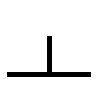
\includegraphics[scale=0.1]{numerals/2.jpg}}
\newcommand{\Nd}{
\includegraphics[scale=0.3]{numerals/3.pdf}}
\newcommand{\Ne}{
\includegraphics[scale=0.3]{numerals/4.pdf}}
\newcommand{\Nf}{
\includegraphics[scale=0.3]{numerals/5.pdf}}
\newcommand{\Ng}{
\includegraphics[scale=0.3]{numerals/6.pdf}}
\newcommand{\Nh}{
\includegraphics[scale=0.3]{numerals/7.pdf}}

\newcommand{\Npos}{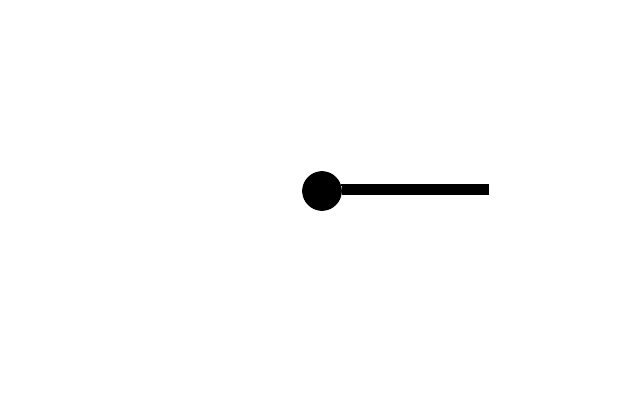
\includegraphics[scale=0.03]{unit/pos.png}}
\newcommand{\Nneg}{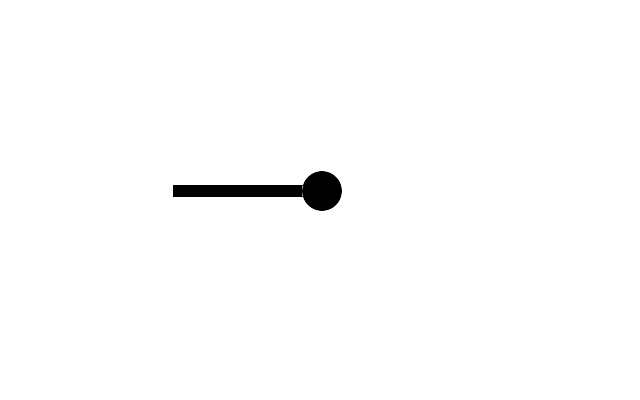
\includegraphics[scale=0.03]{unit/neg.png}}
\newcommand{\Ni}{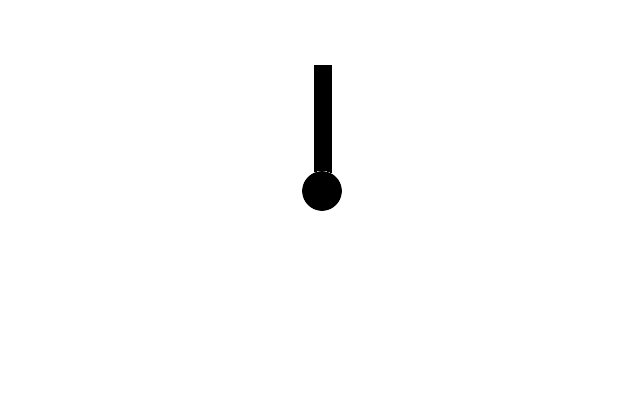
\includegraphics[scale=0.03]{unit/i.png}}
\newcommand{\Nineg}{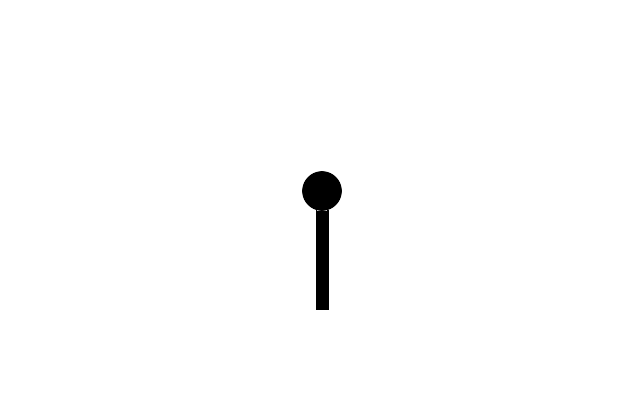
\includegraphics[scale=0.03]{unit/ineg.png}}
\newcommand{\Nang}{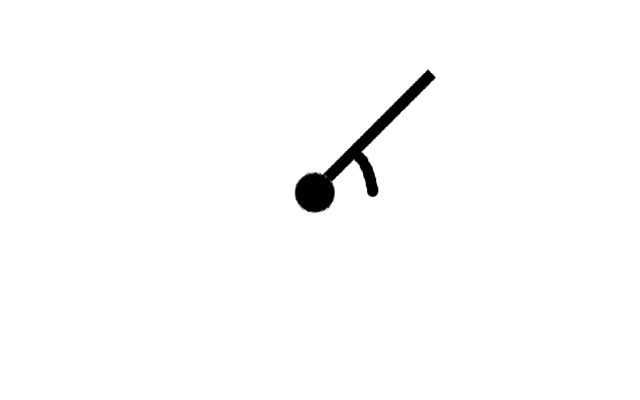
\includegraphics[scale=0.03]{unit/ang.png}}

%\newcommand{\Npi}{\includegraphics[scale=0.02]{trig/2pi.jpg}}
%\newcommand{\Nsin}{
\includegraphics[scale=0.02]{trig/sin.jpg}}
%\newcommand{\Ncos}{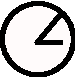
\includegraphics[scale=0.02]{trig/cos.jpg}}
%\newcommand{\Nsec}{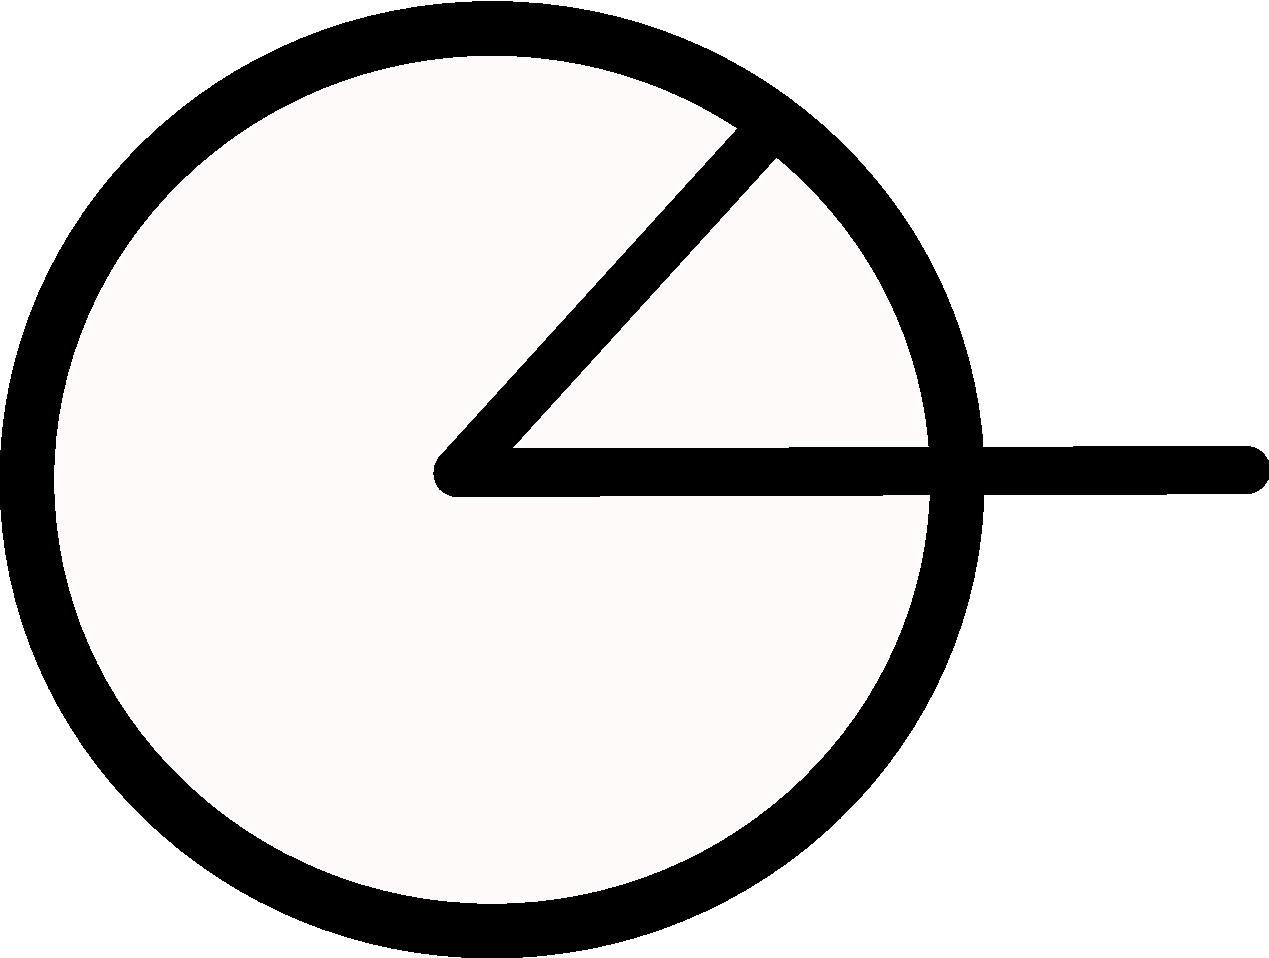
\includegraphics[scale=0.02]{trig/sec.jpg}}
%\newcommand{\Ntan}{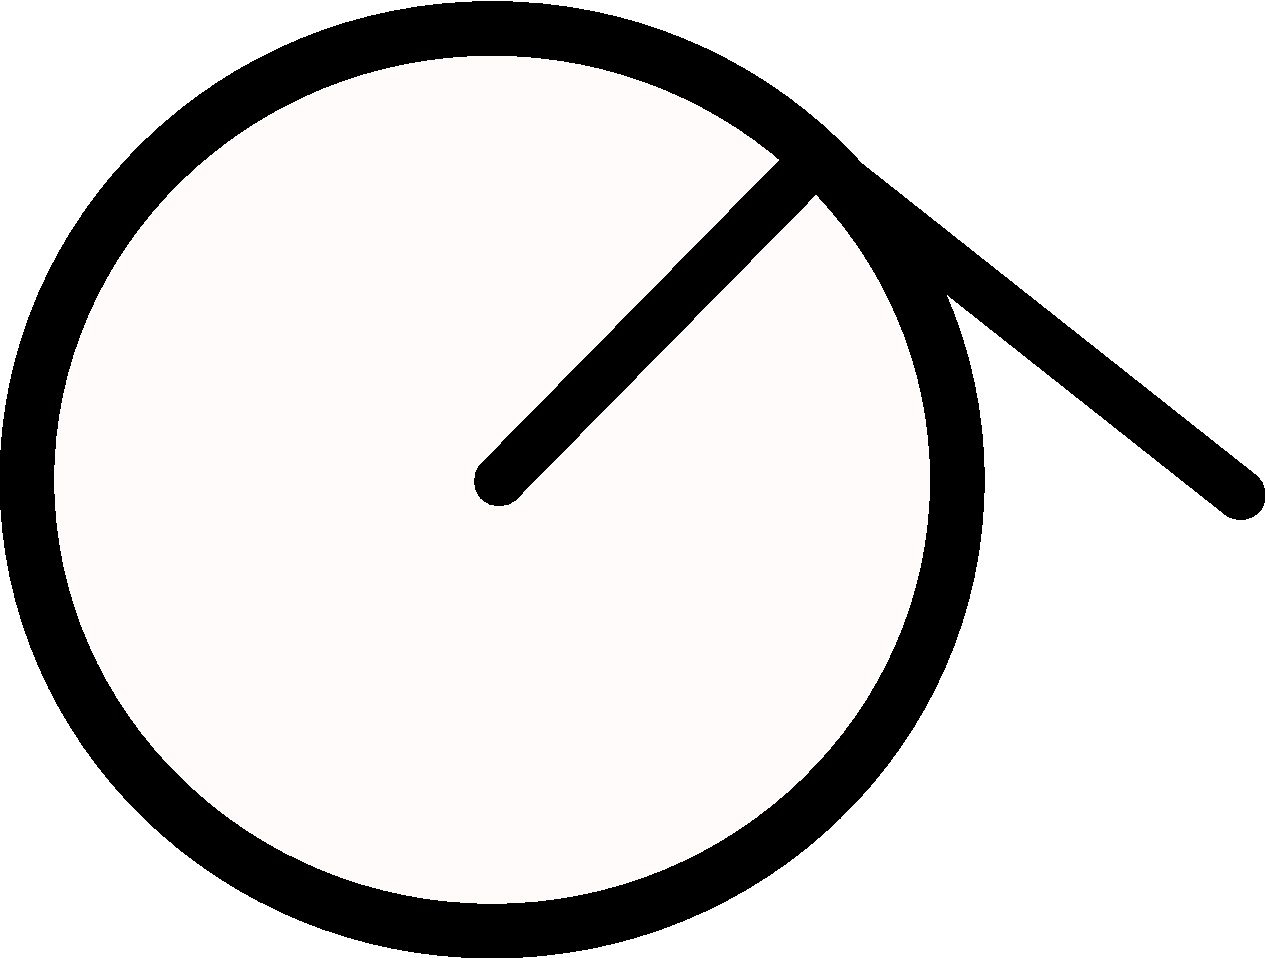
\includegraphics[scale=0.02]{trig/tan.jpg}}
\newcommand{\Npi}{
\includegraphics[scale=0.25]{trig/tau.pdf}}
\newcommand{\Nsin}{
\includegraphics[scale=0.25]{trig/sin.pdf}}
\newcommand{\Ncos}{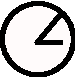
\includegraphics[scale=0.25]{trig/cos.pdf}}
\newcommand{\Nsec}{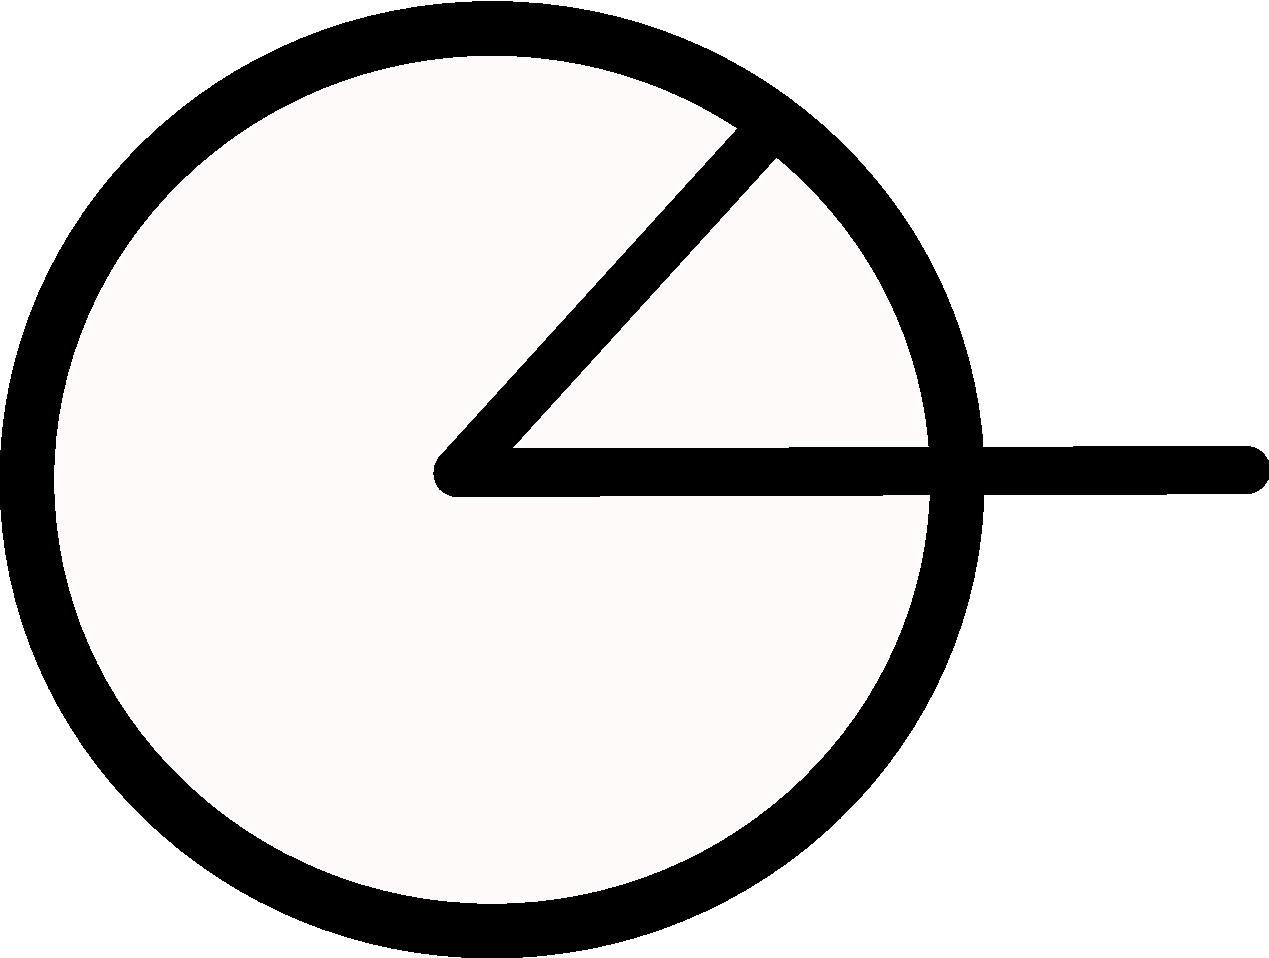
\includegraphics[scale=0.02]{trig/sec.pdf}}
\newcommand{\Ntan}{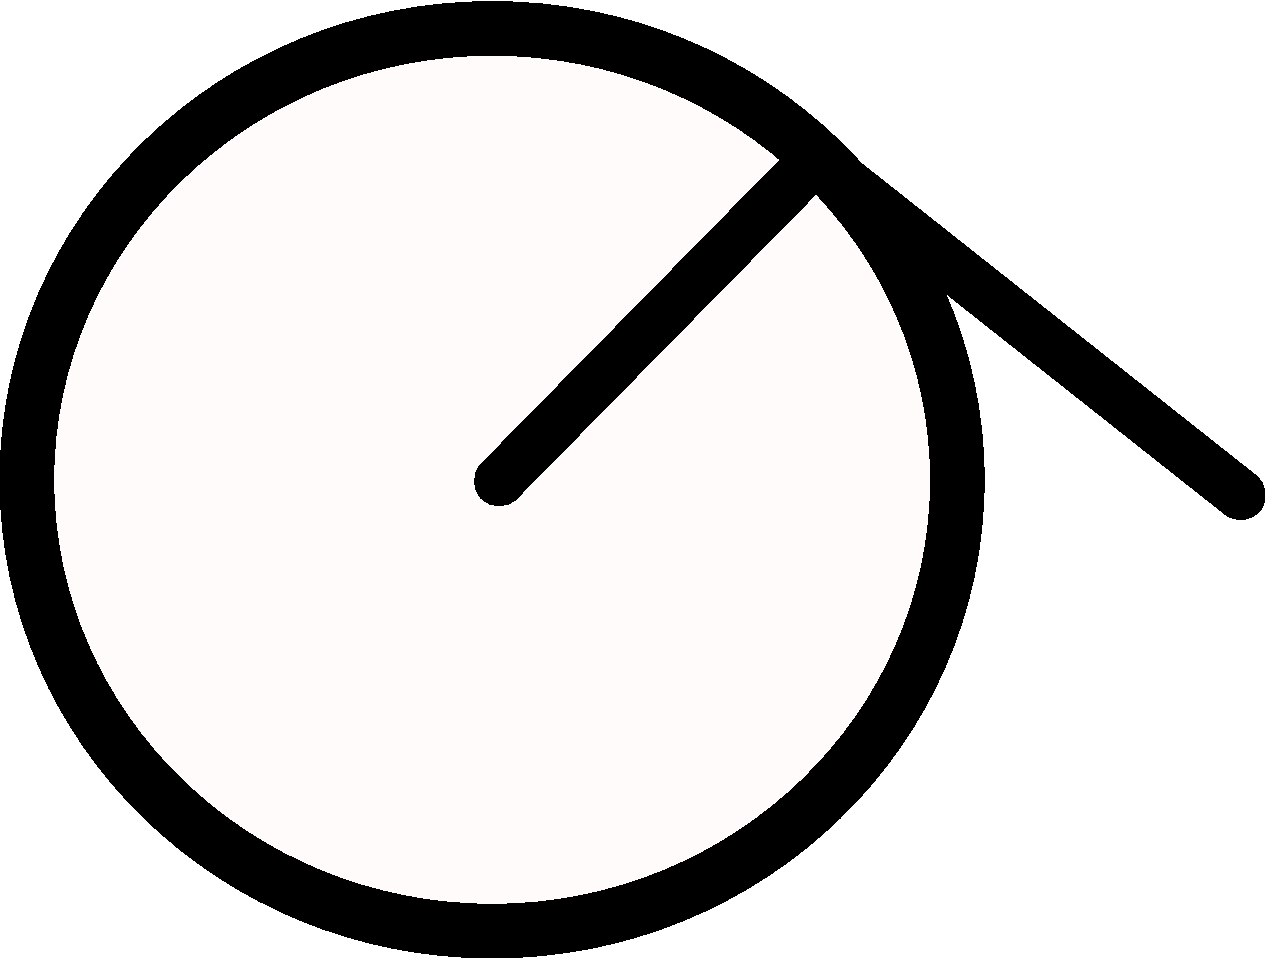
\includegraphics[scale=0.02]{trig/tan.pdf}}



\newcommand{\Nint}{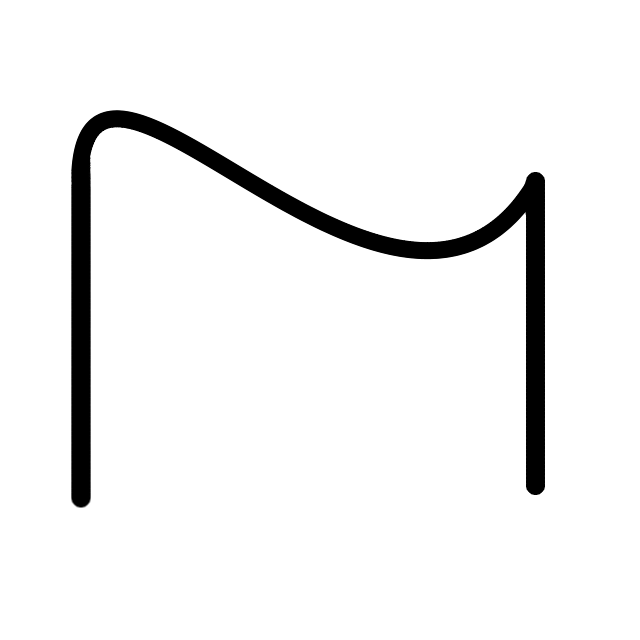
\includegraphics[scale=0.015]{calc/int.png}}
\newcommand{\Ndiff}{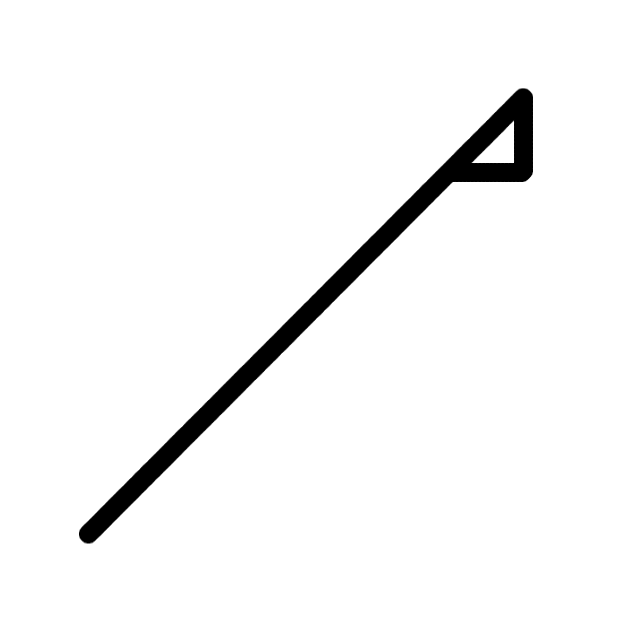
\includegraphics[scale=0.015]{calc/diff.png}}

\newcommand{\Ninter}{
\includegraphics[scale=0.25]{set/inter.pdf}}
\newcommand{\Nunion}{
\includegraphics[scale=0.25]{set/union.pdf}}
\newcommand{\Nsymdiff}{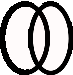
\includegraphics[scale=0.25]{set/symdiff.pdf}}
\newcommand{\Ndisunion}{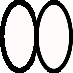
\includegraphics[scale=0.25]{set/dissunion.pdf}}

%\newcommand{\NR}{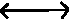
\includegraphics[scale=0.035]{set/R.png}}
\newcommand{\NRp}{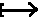
\includegraphics[scale=0.35]{set/R+.pdf}}
\newcommand{\NR}{\longleftrightarrow}
%\newcommand{\NRp}{[\!\to}
%\newcommand{\NN}{\includegraphics[scale=0.035]{set/N.png}}
\newcommand{\NN}{\longleftrightarrow\!\!\!\!\!\!\!\!\shortmid~\!\!\!\shortmid~}
%\newcommand{\NQ}{\includegraphics[scale=0.035]{set/Q.png}}
\newcommand{\NQ}{\Longleftrightarrow\!\!\!\!\!\!\!\!\shortmid~\!\!\!\shortmid~}
\newcommand{\NQp}{
\includegraphics[scale=0.017]{set/Q+.png}}
\newcommand{\NZ}{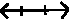
\includegraphics[scale=0.35]{set/Z.pdf}}
\newcommand{\NC}{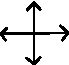
\includegraphics[scale=0.35]{set/C.pdf}}
\newcommand{\NI}{
\includegraphics[scale=0.35]{set/I.pdf}}
\newcommand{\NIZ}{
\includegraphics[scale=0.35]{set/IZ.pdf}}
\newcommand{\NCZ}{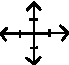
\includegraphics[scale=0.35]{set/CZ.pdf}}


\title{Towards a Better Notation for Mathematics}
\author{Christopher Olah (\hbox{chris@colah.ca})}
\date{July 8, 2010}

\begin{document}

\maketitle

\begin{quotation}

{\bf Abstract:} This paper explores alternative notations for mathematics. We consider numerical notations that make arithmetic easier, a notation for quantifiers that reduces the number of variables one needs to track, and many other ideas.\\

({\bf Regarding Notation:} The typographical quality of new symbols introduced in this paper is terribly lacking -- you will likely need to zoom in on them to see them well. This is because the author is injecting them as images. A font is in the works but isn't much better, as the author is not a skilled font-craft.)\\

{\bf Update:} I've made some minor changes to young-me's work to clean things up a bit. That said, please keep in mind that I've progressed a long way since writing this and it isn't representative of my current abilities.

\end{quotation}

\tableofcontents
\section{Introduction}

When one considers how complicated the ideas mathematical notation must represent are, it clearly does quite a good job. Despite this, the author believes that any claim that modern mathematical  notation is the \emph{best} should be met with extreme scepticism.
 
% %\subsection{An Evolved Language}
% 
Mathematical notation is a natural language: no one sat down and constructed it, but rather it formed gradually by people making changes that are adopted. Most changes are not adopted; whether they are depends on a variety of factors including: mathematical utility, ease of adoption (the average individual doesn't want to spend hours learning), dissemination, and shear dumb luck. The first two of these qualities are associated to real properties in notation, forming the necessary selective pressure for evolution to occur.
 
Evolution is a blind watchmaker: the world around us is filled with examples of the stupidity of biological evolution (the classic example being halibut). Similarly, evolution is also a blind language and notation designer. In particular, it is held back by a strong selective force against change, since people would need to adopt it, and so evolution doesn't effectively explore the full notation-space. This staticism means that even the most outrageous notations remain unchallenged by virtue of age.

% It is absurd to believe that this staticism or even the incremental process of evolution itself are in the best interest of humanity as regards any language, least of all the language of the sciences, the notation of mathematics.
% 
% \subsection{Significance}

The importance of notation is widely recognized in computer science: progress in the design of programming languages over the last few decades has been immense and has been strongly felt by the community. The difference between programming in a legacy language like Fortran and a modern language (Python, Ruby, Haskell, etc) is immense. This idea, that language and notation are important is not an invention of computer science. The Sapir-Whorf hypothesis asserts the language one thinks in effects the way one thinks, and has motivated the creation of many constructed Human languages, such as Esperanto and lojban. But no such intentional language construction seems to be done in mathematics, save perhaps right at the cutting edge of research.

% (Since its inception, mathematical notation has been performing a balancing act between backwards compatibility (so the masses don't have to relearn everything) and needing to be able to handle the new ideas that result from mathematical progress. In modern times, this has only been exasperated as the population of the masses increased and the rate of mathematical progress did likewise. To use a programming language analogy, modern mathematical notation is where python or ruby would be if they tried to maintain backwards compatibility with Fortran -- and continued trying after they inevitably failed.)
% 
% (It goes without saying that this has crippled the potential of mathematical notation.)
% 
% \subsection{Conclusion}
% 
% It is now time for Humanity to throw off the shackles of notations developed by the arbitrary whims of fate and to construct a new notation for mathematics. A better one.
% 
% It is now time for Humanity to take the term `intelligent design' from the rantings of the delusional and turn it into a wilful act of humanity upon our modes of communication.
% 
% Language is our tool. It is time to make notation not be the conveniently shaped stone that was tossed our way by history, but a knife sharpened by the greatest minds we can bring to bare on it.
% 
% The first step towards this is simply to brainstorm about this new notation. 

It may be that the gains of moving to a different notation are so small that they don't justify the cost of switching. But it may also be the case that some notation exists which would greatly increase Human mathematical capabilities. We won't know unless we explore the possibilities.

This paper doesn't assert to be anywhere near the best possible notation. It simply seeks to introduce some interesting ideas. However, before proceeding further and becoming contaminated with these ideas, I would encourage the reader to think about this matter for a few moments: perhaps you will come up with better ideas that can act as the basis for a new and better notation for mathematics.


\section{Version Representation}

In the unrealistic event of this paper inducing mass notation experimentation, there needs to be a way to denote what notation a person is using (while this notation is visually distinctive, this can not be relied on if there are forks). To this end, I propose a version string that can go at the top of a math page. It would begin with ``$MNV\!:$'' (Math Notation Version) followed by the designers handle, an optional branch, and a natural number (all delimited by `.'). For example, the notation described in the final version of this paper can be referred to as:

$$MNV\!:\!colah.1$$

While, if I suddenly started experimenting with using prefix operators, the first version of that notation would be $MNV\!:\!colah.prefix.1$ and I might make the next infix version $MNV\!:\!colah.infix.1$, and which ever one I decided on in the end would become $MNV\!:\!colah.2$.

If the ISO was to endorse a standard, it would be $MNV\!:\!iso.1$ and its successor $MNV\!:\!iso.2$.

The standard notation may be referred to as $MNV\!:\!std$. I leave the naming of historical notations to anthropologists.


\section{Numbers \& Vectors}

$0$, $1$, $2$, $3$, $4$, $5$, $6$, $7$, $8$, and $9$. It takes no deep insight to realise that the Arabic numerals are utterly arbitrary. There is no question that they were superior to the Roman notation that they replaced -- I for one have no desire to try and multiply $VII$ by $XVI$ -- but it does not follow that they should be what we use.

It is important to realise that the great innovation of the Arabic numerals was not the numerals themselves but the technique of representing numbers by wrapping around into the next column (eg. after $9$ comes $10$). This simple system efficiently represents large numbers ($100$ in a unary system: $\cdot\cdot\cdot\cdot\cdot\cdot\cdot\cdot\cdot\cdot\cdot\cdot\cdot\cdot\cdot\cdot\cdot\cdot\cdot\cdot\cdot\cdot\cdot\cdot\cdot\cdot\cdot\cdot\cdot\cdot\cdot\cdot\cdot\cdot\cdot\cdot\cdot\cdot\cdot\cdot\cdot\cdot\cdot\cdot\cdot\cdot\cdot\cdot\cdot\cdot\cdot\cdot\cdot\cdot\cdot\cdot\cdot\cdot\cdot\cdot\cdot\cdot\cdot\cdot\cdot\cdot\cdot\cdot\cdot\cdot\cdot\cdot\cdot\cdot\cdot\cdot\cdot\cdot\cdot\cdot\cdot\cdot\cdot\cdot\cdot\cdot\cdot\cdot\cdot\cdot\cdot\cdot\cdot\cdot\cdot\cdot\cdot\cdot\cdot\cdot$) and allows for easy algorithms for arithmetic. This strategy can be taken with any set of symbols and can even cycle at a number other than $10$ -- this value is called the base and $10$ is mathematically arbitrary. \footnote{It maybe that we use ten because we have ten fingers... (Thanks to Rob Patterson for pointing this out). However, we could also use fingers as binary digits, allowing one to count up to $1024$ on their hands. Or two numbers of sizes up to $32$ and do intuitive addition between them.}

One particularly interesting base is base $2$, called binary. The first column has the possible values of $0$ and $1$, the second $0*2$ and $1*2$ the next $0*2*2$ and $1*2*2$... It has a very elegant addition algorithm: \\

\begin{center}
\begin{tabular}{|c|c|} \hline
Ones & Result\\ \hline
0& 0\\ \hline
1& 1\\ \hline
2& 0, carry\\ \hline
3& 1, carry\\ \hline
\end{tabular}
\end{center}

This can trivially be implemented in logic gates ($xor$ and $and$ are sufficient). It is also very intuitive.

Multiplication is similarly elegant: multiplying by $10000...$ is just phaseshifting and any multiplication can be decomposed into adding the result of such multiplications ($a*(b+c+d)=a*b+a*c+a*d$, after all).

However, elegant and intuitive as it is, binary is slow and tedious (for humans...) because there are so many digits in a binary number. One might wonder if there is a way to keep the intuition of binary while maintaining the speed and ease of a higher base system.

What if we were to group binary numbers to form numerals? This can be done to form any $2^n$ base, but we select octal (base 8). (The choice over hexadecimal is motivated by ease of learning -- $256$ items in the multiplication table is insane -- and for improved visual differentiation of numerals).\footnote{Another nice feature of octal is that the base -- significant because the base used seems to become the most pleasant number in most people's mind -- is two cubed and thus factorable three times, a far nicer number to work with.}

Thus the symbols are:\\

\begin{center}

\begin{tabular}{|c|c|}\hline
\multicolumn{2}{|c|}{Numerals}\\ \hline
Standard & Proposed\\ \hline
$0$ & \Na\\
$1$ & \Nb\\
$2$ & \Nc\\
$3$ & \Nd\\
$4$ & \Ne\\
$5$ & \Nf\\
$6$ & \Ng\\
$7$ & \Nh\\ \hline
\end{tabular}\\

\end{center}

For example $\Ne + \Nd = \Nh$ and $\Nc * \Nd = \Ng$.

The next obvious question is how to represent negative numbers. A natural notation can be derived from the geometric interpretation of such numbers:\footnote{Lines coming out of a dot were chosen over arrows to reduce the number of strokes involved in writing numbers... and to reserve them for other uses.}\footnote{One mild concern is that the directions of the unit vectors conflict with the directions of the base powers (ie. that the powers of the columns go $...2^3 2^2 2^1 2^0 2^{-1} 2^{-2} 2^{-3}...$, decreasing from left to right, while the unit vectors have positive in the right direction). People seem to find it highly disconcerting to change these conventions, but I am considering doing so anyway.}

\begin{center}
\begin{tabular}{|c|c|}\hline
\multicolumn{2}{|c|}{Numerals}\\ \hline
Standard & Proposed\\ \hline
$+1$  & \Npos \Nb \\
$-1$ & \Nneg \Nb\\ \hline
\end{tabular}\footnote{To me, there is a distinction between $+1$ and $1$: $1$ is a natural number, a cardinality, while $+1$ is a integer or maybe even complex number that happens to have the value of a natural number. Thus, I don't think a positive unit vector is out of place.}\footnote{\Nb $~$ is purely superficial.}\\
\end{center}

This naturally scales to all complex numbers:

\begin{center}
\begin{tabular}{|c|c|}\hline
\multicolumn{2}{|c|}{Numerals}\\ \hline
Standard & Proposed\\ \hline
$+1$  & \Npos \Nb  \\
$i$ & \Ni \Nb \\
$-1$ & \Nneg \Nb \\
$-i$ & \Nineg \Nb \\ \hline 
\end{tabular}\\
\end{center}

It would be nice to be able to create complex unit numbers of an arbitrary argument. To this end we will introduce the notation $\!\!\!\!\!$\begin{tabular}{l}\Nang\vspace{-0.4cm}\\ $~~_\theta$\\\end{tabular}$\!\!\!\!\!$ as equivalent to $e^{i\theta}$.

What about vectors though? They can have more than two dimensions... We will use $\!\!\!\!\!$\begin{tabular}{l} $~~^n$ \vspace{-0.1cm}\\ \Ni \\ \end{tabular}$\!\!\!\!\!$ to represent the $n$th unit vector.




\section{Sets}

Firstly, some new symbols for the standard sets. They are constructive symbols -- there are obvious rules that allow one to create many sets that do not usually have symbols.\\

\begin{center}
\begin{tabular}{|c|c|} \hline
$\NN$ & $\mathbb{N}$\\ \hline
$\NZ$ & $\mathbb{Z}$\\ \hline
$\NQ$ & $\mathbb{Q}$\\ \hline
$\NQp$ & $\mathbb{Q}^+$\\ \hline
$\NR$ & $\mathbb{R}$\\ \hline
$\NRp$ & $\mathbb{R}^+$\\ \hline
\end{tabular} $~~~$
\begin{tabular}{|c|c|} \hline
$\NC$ & $\mathbb{C}$\\ \hline
$\NI$ & $\mathbb{I}$\\ \hline
$\NIZ$ & $\{ai | a \in \mathbb{Z}\}$\\ \hline
$\NCZ$ & $\{a+bi | a,b \in \mathbb{Z}\}$\\ \hline
$...$ & $...$\\ \hline
\end{tabular}
\footnote{The notation for $\mathbb{R}$ (the origin of this strategy) was proposed by Rob Gibson and lead to this strategy. The notation for $\mathbb{Q}$ was proposed by Adina Bogert-o Briea. }
\end{center}

It is my belief that we could benefit from some standard classes for the classes of things like sets, open sets, closed sets, compact sets (or variants), topological spaces, topological spaces that meet certain separation axioms, et cetera. For now, I will use $\{s\}$ to denote these (eg. the class of sets is $\{set\}$ which is actually, apparently, somewhat used).\footnote{Some tempting notations here would not be practical to handwrite. For example, an open set could be a filled circle with soft edges... The idea of having special symbols for typeset documents bares consideration in the computer age.}


Drawing off the notation of Venn Diagrams, the notation for intersections and unions will be $\Ninter$ and $\Nunion$ as opposed to $\cap$ and $\cup$. A disjoint union can be represented by $\Ndisunion$ and a symmetric difference by $\Nsymdiff$ as opposed to $\sqcup$ and $\Delta$ respectively.

For Cartesian products, I propose $\square$, given the intuitive representation of all possible pairs as a rectangle.

\section{Boolean Operations}

Boolean operations extend naturally from set operations. If we consider false to be the empty set $\{\}$ and true to contain an element $t$, $\{t\}$, intersection forms the and truth table, union or, and symmetric difference exclusive or.

These same symbols naturally extend to their fuzzy logic equivalents.

\section{Standard Functions}

It is possible to achieve many vital operations by applying the hyper operation and functional exponentiation to the increment operator, $inc$. Intuitively, the hyper operation takes a operation and creates a new one by applying the operation to a value $a$, $b$ times. More formally:


$$ \begin{array}{l}  hyp: $~~~$ (A^m \to A) $~$ \to $~$ (A\times\mathbb{N} \to A)\\
 hyp(f) = \left\{\begin{array}{ll} 
a,n \to f^n(a) & m = 1\\
a,n \to (x \to f(a,x))^{(n-1)}(a) & m = 2\\
... & ... \\
 \end{array}\\ \end{array}$$

Furthermore, we will define $inv$ as the inverse function (ie. $f \to f^{-1}$) and $inv_n$ as the inverse function with respect to the $n$th variable in a multivariable function. $hyp_n$ specifies that the $n$th variable is the repeated one. Then $hyp$ and the $inv$s can, from $inc$, form many important functions:\\

$\!\!\!\!\!\!\!\!\!\!\!\!\!\!\!\!\!\!\!\!\!\!\!\!\!\!\!\!\!\!\!\!\!\!\!\!\!\!\!\!\!\!\!\!\!\!\!\!\!\!\!\!$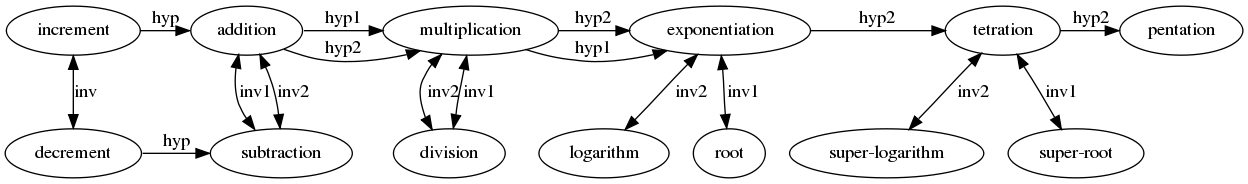
\includegraphics[scale=0.4]{hyperfunctions.png}\\

We might use a shorter symbol for $inc$, say $+$, and allow subscript to be the application of $hyp$, applied before functional exponentiation. Then addition is $+_{\Nb}$ ($+_1$), multiplication $+_{\Nc}$ ($+_2$) and so on.

However, this is somewhat unruly to work with, so we might prefer to create some other operators. Since the natural numbers are the sizes of sets, a natural parallel between set operations and many of the operations we are seeking symbols for forms.


Since, for sets of size $a$ and $b$, the size of the disjoint union is the sum of $a$ and $b$, it is intuitive that the same symbol be used for union and addition. Thus, the symbol for addition is $\Ndisunion$.

Similarly, since, for sets of size $a$ and $b$, the size of the cartesian product is the product of $a$ and $b$, the symbols for multiplication should be $\square$. This is also intuitive in that the area of a rectangle with sides of lengths $a$ and $b$ is the product of them. Alternatively, the direct operator performs multiplication where valid (see unit vectors).

Exponentiation and functional exponentiation will continue to be superscripts since we were using this in our $hyp$ based notation (and the author doesn't have any better ideas -- we might do something like Knuth's up arrows ($\square_n$ is tempting), but it would be rather tedious for polynomials).


An inverse for addition is unnecessary, since we have a negative unit vector. There is not presently a good symbol proposed for division.


\section{Trigonometry}

The notation I propose for trigonometry is inspired by the visualisation of trigonometry on the unit circle:\\


$\!\!\!\!\!\!\!\!\!\!\!\!\!\!\!\!\!\!\!\!\!\!\!\!\!\!\!\!\!\!\!\!\!\!\!\!\!$\begin{tabular}{|c|c|c|c|}\hline
Standard Symbol & Proposed Symbol & Standard Read & Proposed Read \\ \hline
$2\pi$ & \Npi & Two Pi & Turn \\  \hline
$\cos$ & \Ncos & Cosine & Adjacent [Projection] (of Angle)\\  \hline
$\sin$ & \Nsin & Sine & Opposite [Projection] (of Angle)\\  \hline
$\tan$ & \Ntan & Tangent & (Angle) Tangent\\  \hline
$\sec$ & \Nsec & Secant & Reciprocal Adjacent [Projection] (of Angle)\\  \hline
... & ... & ... & ... \\ \hline
\end{tabular}$~$\footnote{Regarding $2\pi$: see \href{http://www.math.utah.edu/~palais/pi.html}{$\pi$ is wrong} and \href{http://tauday.com/}{The Tau Manifesto} (from which the name turn is taken) for justifications; the matter has been dealt with at length there.}\footnote{One person who saw this notation believed they had seen it elsewhere but was uncertain as to where. I have not been able to find it.}\\

In addition to making all the symbols obvious (no more memorisation! take that, sohcahtoh!), this notation makes a number of trigonometric identities into painfully obvious corollaries of Pythagoras' Theorem; for example:

$$(\Ncos a)^2 + (\Nsin a)^2 = 1^2$$

$$(\Nsec a)^2 + 1^2 = (\Ntan a)^2$$


\section{Calculus}

The notation I propose for calculus is differential forms with a different operator.

For those unfamiliar with differential forms, it is a slight nuance of Leibniz notation; if $f(x)=x^2$:

\begin{center}
\begin{tabular}{|c|c|c|}\hline
Newton & Leibniz & Differential forms\\\hline
$f'(x) = 2x$ & $\frac{d}{dx} x^2 = 2x$ & $dx^2=2xdx$\\\hline
\end{tabular}\\
\end{center}

This is great for working with multiple variables and leads to elegant formulations of the differentiation rules (eg. $duv = udv + vdu$). On the other hand, the symbol $d$ is rather arbitrary; I propose we use \Ndiff, the idea being that it is the tiny bit of change at the end. For example: $\Ndiff x^2 = 2x \Ndiff x$.

For integral, the best symbol I can come up with is \Nint, but I am rather discontent with it. Of course, if one just wants to antidifferentiate, $\Ndiff^{-1}$ is perfectly valid.

\section{Quantifiers}

Qualified statements are often tedious to write. For example, I find $(\forall a \in \mathbb{R})(\forall b \in \mathbb{R})(\exists c \in \mathbb{R})(a+b=c)$ to be absurdly verbose. The problem isn't the physical space it occupies but the conceptual space it occupies: I want to say ``the sum of two real numbers is a real number" not "for any real number $a$ and any real number $b$ there exists a real number $c$ such that $a$ plus $b$ equals $c$." So I propose the alternative: $\mathbb{R}^\forall +\mathbb{R}^{\forall'} = \mathbb{R}^\exists$.

This notation allows for one to more closely approximate the idea behind different mathematical concept.

The idea behind limits isn't $\lim_{x\to p} f(x) = V \iff (\forall \epsilon > 0)(\exists \delta >0)( |x-p| < \delta \rightarrow |f(x) - V| < \epsilon$ -- ``The limit as $x$ tends to $p$ of $f(x)$ is $V$ if and only if for every $\epsilon$ greater than zero there exists $\delta$ greater than zero such that the difference between $x$ and $p$ being less than $\epsilon$ implies than difference between $f(x)$ and $V$ is less than epsilon.'' It's much closer to $\lim_{x\to p} f(x) = V \iff {\mathbb{R}^+}^\forall > V - f(B_{\mathbb{R}^\exists}(p)^\forall)$ -- ``The limit as $x$ tends to $p$ of $f(x)$ is $V$ if and only if for every positive real number there is a ball around $p$ with every point in it being mapped by $f$ to a value less than that much different from $V$.''

The idea Hausdorff spaces isn't $(\forall p_1, p_2 \in X; p_1\neq p_2)(\exists u,v \in \{open\}, p_1\in u, p_2 \in v)(u\cap v = 0)$ -- ``For any point $p_1$ and any different point $p_2$ there exists open sets $u$ around $p_1$ and $v$ around $p_2$ such that $u$ and $v$ don't intersect.'' It's $\{open\}(X^\forall)^\exists \cap \{open\}(X^{\forall'})^\exists = 0$ -- ``Any two different points have disjoint open sets around them.''

This isn't to say that the $(\forall...)(...)$ and $(\exists...)(...)$ notations are always worse. There are some circumstances where they are better and thus it makes sense to keep them as complements to these anonymous qualifiers. Of course, the symbols need to be replaced... Suggestions are appreciated.



\section{Science}

It would be absurd to change mathematics without consideration to the needs of scientists; they're probably the primary users of mathematics, outside the arithmetic used in every day life by most people. 

The author can only comment as an outside observer.

It is striking that scientists like to clutter the namespace, not even regarding the ways they conflict with each other... Just about every variable is occupied by some meaning, often by many.

One of the more egregious examples is the notation for fields in physics. Rather than using one symbol plus subscripts as in forces, they choose to use a unique symbol for each one ($E$, $B$...). Similarly, is it really necessary for each derivative of distance to have its own symbol? Furthermore, is it really not possible to come up with better symbols than letters that have vague anglocentric relations to the represented value?

\section{Equality, Scope \& Algebra}

When someone writes $=$, I am often not sure what they mean. Are they asserting that two things are equal? Defining one to be the other? Is it a boolean equality test? These are all very distinct.

In programming languages, assignment and equality testing are usually assigned to different operators (eg. C: $=$ and $==$); similarly, some mathematicians choose to use $:=$ for their assignment operator. However, even then there is some ambiguity: most of these assigned variables are local, but there is no such signification or anyway to describe the bounds of their scope.

Finally, there is the mystery of what is intended by things like:

$$x^2 +1 = 5$$
$$x^2 = 4$$
$$x = \pm \sqrt{4}$$
$$x = \pm 2$$

What is intended here? It isn't clear to me that somewhat is asserting any of the statements to be true (with more context, they may be), but rather it seems to be a \emph{suppose that... then...} scenario. So what is actually being conveyed?

$$x^2 +1 = 5$$
$$\updownarrow$$
$$x^2 = 4$$
$$\updownarrow$$
$$x =  \sqrt{4} \textrm{ or } x = - \sqrt{4}$$
$$\updownarrow$$
$$x =  2 \textrm{ or } x = -2$$

It strikes me that this sort of explicit logical description is beneficial both to reader and author.


\end{document}

